\begin{frame}{¿Por Qué Minimizar la Masa en Aplicaciones Aeroespaciales?}
  \begin{block}{El Desafío del Reactor Espacial}
    \begin{itemize}
      \item El objetivo principal es encontrar un material que ofrezca la
        protección necesaria contra la radiación con la \textbf{mínima masa
        posible}.
      \item Esto es un problema de optimización donde se busca la mayor
        eficiencia de blindaje por unidad de masa.
    \end{itemize}
  \end{block}
  \begin{block}{Índice de Material a Optimizar}
    Para este problema, maximizamos el índice de masa mínima:
    $$ \mathcal{M}_{2} = \frac{\lambda_{eff}}{M} $$
    Donde $\lambda_{eff}$ es la atenuación y $M$ es la masa molar.
  \end{block}
\end{frame}

\begin{frame}
  \begin{figure}
    \centering
    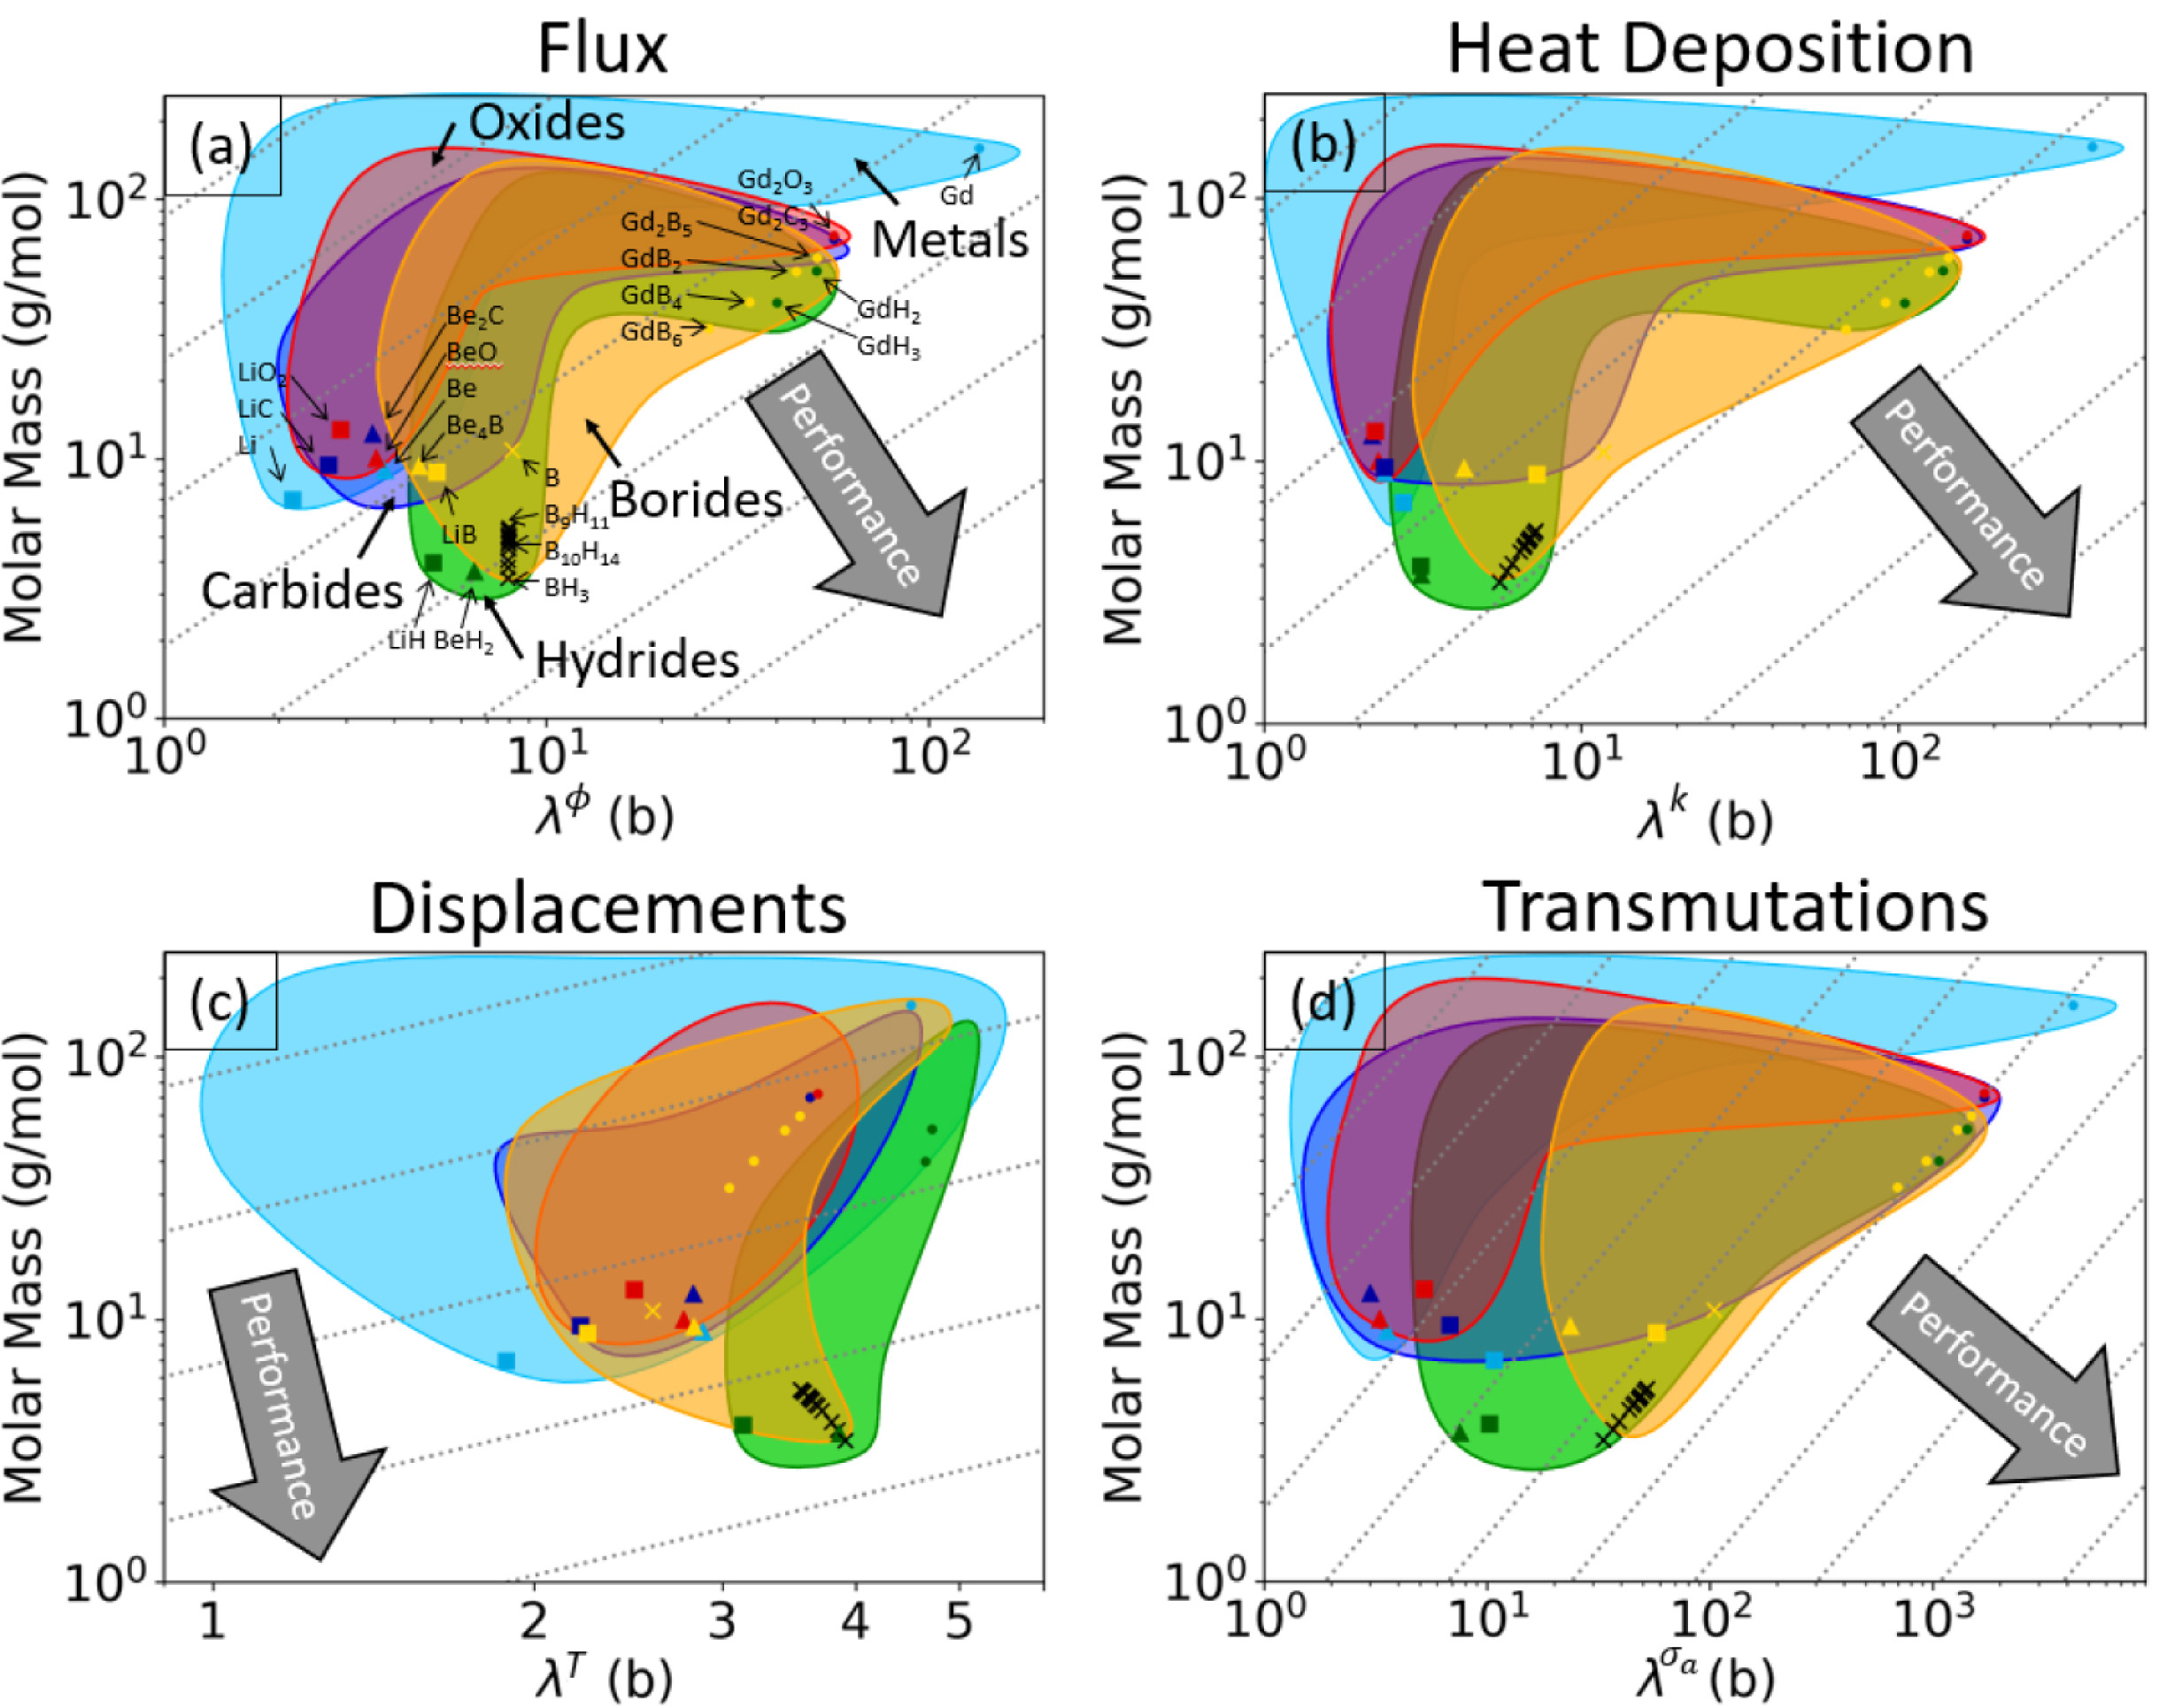
\includegraphics[width=0.65\linewidth]{../images/graph-4.jpg} 
    \caption{Materiales para blindaje de masa mínima, protegiendo
    \ce{Si} de un espectro de fisión rápido. \cite{Brand2025Material}}
  \end{figure}
\end{frame}

\begin{frame}
  \frametitle{El Material Óptimo para Proteger el Chip}
  \begin{block}{Recordando el Objetivo}
    Buscamos el material con el mayor \textbf{Índice de Material} para minimizar la masa:
    $$ \mathcal{M}_{2} = \frac{\lambda_{eff}}{M} \rightarrow \text{Maximizar}$$
  \end{block}

  \begin{alertblock}{Los Candidatos Ganadores}
    Los \textbf{Boranos} (compuestos de Boro e Hidrógeno, como \ce{B10H14}) y
    los \textbf{Hidruros} (como LiH) son los mejores materiales, superando a
    opciones más convencionales.
  \end{alertblock}
\end{frame}

\begin{frame}
  \begin{block}{¿Por Qué Son los Mejores? La Razón detrás de $\mathcal{M}_{2}$}
    \begin{itemize}
      \item \textbf{Hidruros (\ce{LiH})}: Son extremadamente ligeros (minimizan
        '$M$') y el hidrógeno es un excelente moderador de neutrones.
      \item \textbf{Boranos (\ce{B_xH_y})}: Ofrecen la mejor combinación. Tienen
        una masa molar muy baja ($M$) y un coeficiente de atenuación
        ($\lambda_{eff}$) excepcionalmente alto. Esto se debe al
        efecto combinado de la \textbf{alta absorción} de neutrones del Boro y
        la \textbf{alta dispersión} del Hidrógeno.
    \end{itemize}
  \end{block}
\end{frame}
